\graphicspath{{content/chapters/7_evaluation/figures/}}
\chapter{Evaluation}
\label{chp:evaluation}

This chapter provides a comprehensive evaluation of the implemented speech enhancement pipeline. The analysis is divided into three major parts: (i) a comparison of dataset handling strategies and their impact on computational efficiency, (ii) an assessment of model performance across dataset variants, and (iii) hyperparameter tuning on the best-performing dataset–model configuration. This layered evaluation approach enables both system-level insight and fine-grained model optimization.

\section{Dataset Performance}
\label{sec:dataset_performance}

This section examines the performance of the three dataset handling strategies—Static Bucketing, Dynamic Bucketing, and Padding-Truncation Output-Truncation (PTO). The goal is to assess how these strategies affect the overall efficiency of the training process, particularly in terms of dataset loading times, runtime overhead during training, and their influence on model performance. Each strategy was tested using the same model architecture, the Contextual Encoder-Decoder (CED), under two conditions:

\begin{itemize}
    \item \textbf{Cold Run (Uncached):} In this scenario, all dataset operations are executed from scratch. Static and Dynamic Bucketing compute bucket assignments (with Dynamic Bucketing also requiring K-Means clustering), while PTO calculates and stores the original waveform lengths. This setup simulates a first-time deployment or training on a fresh system.
    
    \item \textbf{Warm Run (Cached):} This run utilizes cached data generated during the cold run, significantly reducing load and preprocessing time. For Static and Dynamic Bucketing, bucket mappings and K-Means centers are reloaded. For PTO, the previously computed original sequence lengths are retrieved.
\end{itemize}

The configuration used for all runs is shown in Figure~\ref{fig:dataset_config}, with the only varying parameter being the \texttt{PAD\_METHOD}.

\begin{figure}[H]
    \centering
    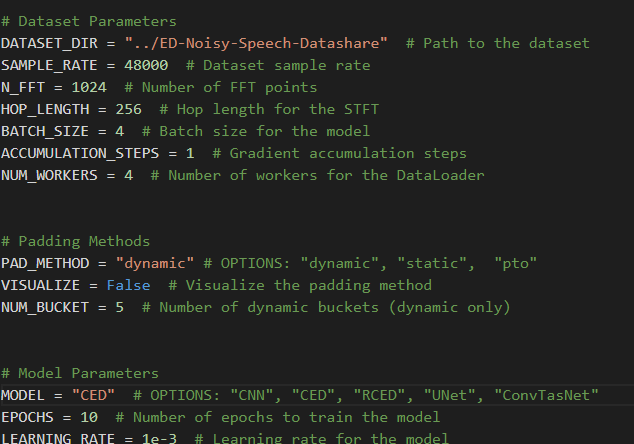
\includegraphics[width=0.8\textwidth]{dataset_config.png}
    \caption{\label{fig:dataset_config} Configuration of the CED model used for dataset performance evaluation.}
\end{figure}

Both uncached and cached runs were executed, and the relevant timing metrics were collected from the output logs, as shown in Table~\ref{tab:dataset_loading_times}.

\vspace{1em}
\begin{table}[H]
\centering
\caption{Training dataset preparation and runtime overheads (in seconds)}
\label{tab:dataset_loading_times}
\begin{tabular}{|l|c|c|c|}
\hline
\textbf{Dataset Type} & \textbf{Initial Load (Uncached)} & \textbf{Re-run Load (Cached)} & \textbf{Epoch Truncation Overhead (PTO only)} \\
\hline
Static Bucketing  & 298.05  & 0.81  & N/A    \\
Dynamic Bucketing & 602.56  & 0.58  & N/A    \\
PTO               & 311.21  & 0.58  & 58.56  \\
\hline
\end{tabular}
\end{table}

The results in Table~\ref{tab:dataset_loading_times} offer a clear overview of the dataset loading times and runtime overheads associated with each method. Static Bucketing proves to be the fastest in terms of initial load time, comprising only dataset loading and bucket assignment. Dynamic Bucketing incurs the highest overhead due to the computational cost of K-Means clustering. PTO, while slightly slower than Static Bucketing, remains efficient given that it must iterate through the dataset to compute the original waveform lengths.

The re-run loading times for all three methods are drastically reduced thanks to the use of cached data. All methods show comparable re-run times, with Static Bucketing being marginally slower.

A key distinction lies in the \textit{epoch truncation overheads}. Only the PTO method incurs this overhead due to its need to truncate outputs during training and evaluation to match the original input lengths. This step is unnecessary for the other two methods. While the added runtime is relatively minor in the context of total training time (typically in the order of hours), this overhead can scale significantly with larger datasets or more training epochs.

To evaluate the impact of dataset handling strategies on model learning, all models were compared using their best training checkpoint. Since the difference between cached and uncached runs was negligible in terms of performance, only the cached results are reported in Table~\ref{tab:dataset_performance}.

\vspace{1em}
\begin{table}[H]
\centering
\caption{Model Training Performance Across Dataset Handling Strategies}
\label{tab:dataset_performance}
\begin{tabular}{|l|c|c|c|}
\hline
\textbf{Dataset Type} & \textbf{Training Loss} & \textbf{Validation Loss} & \textbf{Validation SNR} \\
\hline
Static Bucketing  & 0.8367  & 0.8410  & 1.09 dB \\
Dynamic Bucketing & 0.8262  & 0.8298  & 1.10 dB \\  
PTO               & 0.6288  & 0.6633  & 1.10 dB \\
\hline
\end{tabular}
\end{table}

The results in Table~\ref{tab:dataset_performance} indicate that the model achieves comparable performance across all dataset handling methods. The consistent validation SNR values confirm that each method was implemented correctly and that the model learned similar representations regardless of the input formatting.

Interestingly, the PTO method shows a slightly lower training and validation loss. This discrepancy is not reflected in the SNR metric and may be attributed to differences in how output sequences are truncated during training. The closeness of training and validation losses across all configurations suggests that the model generalizes well and is neither underfitting nor overfitting.
